\documentclass{article}
\usepackage[utf8]{inputenc}
\usepackage{amsmath, amssymb, amsthm}
\usepackage{comment}
\usepackage{graphicx, float}
\usepackage[spanish, es-tabla]{babel}
\graphicspath{{C:\Archive\LaTeX Works\Servicio Social\Reporte 1}}

\title{Reporte 1 Servicio Social}
\author{Carlos Monjaraz}
\date{09/09/2026}

\begin{document}

\maketitle


\section{Investigación sobre flujos óptimos de potencia en sistemas monofásicos y trifásicos usando OpenDSS}
adadas
\section{Como realizar una simulación en OpenDSS}
Por medio de la documentación del programa OpenDS y a través de la
lista de videos en el canal de EPRI OpenDSS para aprender a simular 
en OpenDSS, logré aprender las diferentes funcionalidades básicas del programa,
como lo es la sintaxis, verbos de comando básicos y como se declaran los parámetros 
en el programa.

Por ejemplo, en la carpeta de ejemplos del programa se tienen varios casos de estudio simples,
como lo es el caso de "37Bus", en el cual se presentan los siguientes parámetros:

Primero en el ejemplo se declara un nuevo "objeto" llamado \textit{circuit.ieee37} (esto a través del 
comando "New"), además le agrega varias especificaciones

A su vez aparecen varias líneas de comandos, algunas son para el transformador de la subestación, otra
para el transformador de la carga, y después varias líneas que representan a las líneas de trasmisión eléctrica,
declarando cosas como fases, la longitud y los buses 1 y 2.
Después realiza lo mismo con las cargas, pero agregando el voltaje, y potencia activa y reactiva.

Ya por ultimo está la línea con la que el programa se encarga de resolver el circuito y las iteraciones que usará.

Para ejecutar el programa el usuario debe seleccionar la parte del código que quiere ejecutar, en este caso todo el
código (para seleccionar todo de manera rápida es muy útil usar la combinación de teclas Ctrl+A), después de seleccionar
todo el código se tienen varias opciones para ejecutarlo, como lo es buscar en la interfaz la pestaña "Do" y seleccionar la
primera opción, o lo que es más cómodo usar la combinación de teclas Ctrl+D teniendo todo seleccionado.


%In 1902, Einstein created this famous equation: $E=mc^2$
%Newton came up with: $\sum F=ma$

\begin{equation}
    5+5=10
\end{equation}

\begin{equation}
    \begin{split}
        A & = \frac{\pi r^2}{2} \\
        A & = \frac{1}{2} \pi r^2
    \end{split}
\end{equation}

%How to add images

\begin{figure}[H]
\centering
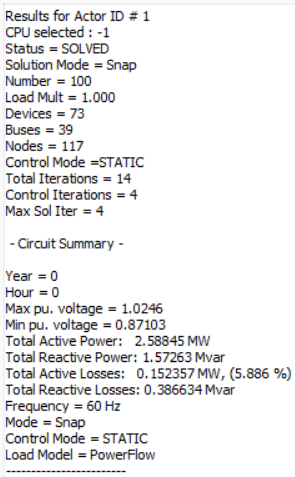
\includegraphics[width=3in]{Resul_Simul_37Bus.png}
\caption{Resultados de la simulación del ejemplo}
\label{fig:my_label}
\end{figure}

Como se puede observar en la anterior figura, OpenDSS da un resumen del circuito.

\end{document}